\addchapheadtotoc
\chapter{An approach to automated testing using a Requirement Automation Tool (RAT)}

This chapter describes the tools and standards used in the current manual testing approach and illustrates the importance of SecurityRAT.

\section{Current testing workflow}
\label{current_testing_etas}

\subsection{Open Web Application Security Project (OWASP)}
The Open Web Application Security Project, short OWASP \citep{owasp2020}, is a non-profit organization that aims to improve web application security by providing freely available educational material. The material includes different tooling, on-demand videos, forums, and extensive documentation. 
The OWASP project is mostly known through the open-source projects, created and maintained by the community.
One of their most famous projects is the OWASP Top 10 \citep{owaspTopTen2020}, which lists the most common vulnerabilities for web applications. The Application Security Verification Standard \citep{owaspAsvs2020} is another of OWASP's popular flagship projects. 


\subsection{Application Security Verification Standard (ASVS)}
\label{asvsStandard}
The Application Security Verification Standard, short ASVS, is a community-driven project that aims to provide a baseline of security controls for web application testing.
It was developed with two main uses in mind. 
As a metric, it supports developers to estimate the "degree of trust" \citep{asvs4.0} that can be placed in their applications.
As a guide, it provides a base for application security requirements in contracts. It tells developers what security controls need to be built into the application to comply with the given requirements.

ASVS can be used to establish a level of confidence in the security of Web applications \citep{asvs4.0}. This is achieved by defining three levels, which are categorized as follows.

\begin{itemize}
    \item Level 1 is for low assurance levels and is completely penetration testable. 
    
    \item Level 2 is for applications that contain sensitive data, which requires protection and is the recommended level for most apps.
    
    \item Level 3 is for the most critical applications - applications that perform high-value transactions, contain sensitive medical data, or any application that requires the highest level of trust.
\end{itemize}
\citep{asvs4.0}

\subsection{Cloud Computing Compliance Controls Catalogue (C5)}
The C5, published by the Federal Office of Information Security, provides a set of criteria to assess the information security of cloud services \citep{bsiC5}.
Since there is no defacto standard, only several context-specific standards, C5 aids customers to get an overview at a higher level of security. 

It is divided into 17 sections that define requirements for different domains, including standard information security entities like "Cryptography and key management", and also more organizational domains like "Personnel", which assures that employees are aware of their responsibilities and the confidentiality of the assets they handle. 

C5 itself builds on top of national and international standards such as ISO/IEC 27001, the Cloud Controls Matrix, the BSI IT-Grundschutz, and German standards such as BSI SaaS Sicherheitsprofile \citep{bsiC5}.

\subsection{OWASP SecurityRAT}
The OWASP Security Requirement Automation Tool, short SecurityRAT, is an application designed to streamline the management of security requirements throughout the development process.
It comes with an initial set of requirements stated in the ASVS. Users, however, are encouraged to create their own set of requirements since risk profiles differ significantly between companies.
SecurityRAT emphasizes automation over merely listing requirements. Properties of an application in development are specified, then used to filter down the set of requirements only to get the ones that have to be fulfilled. 

The set of requirements, for example, contains elements specific to Microsoft Azure Implementation. Each "Implementation Type" has it is own given set of requirements.

\newpage

The requirements can be annotated about whether they have to be implemented or not. In addition to that, the reasoning or result can be documented in SecurityRAT.

\begin{figure}[ht!]
\begin{center}
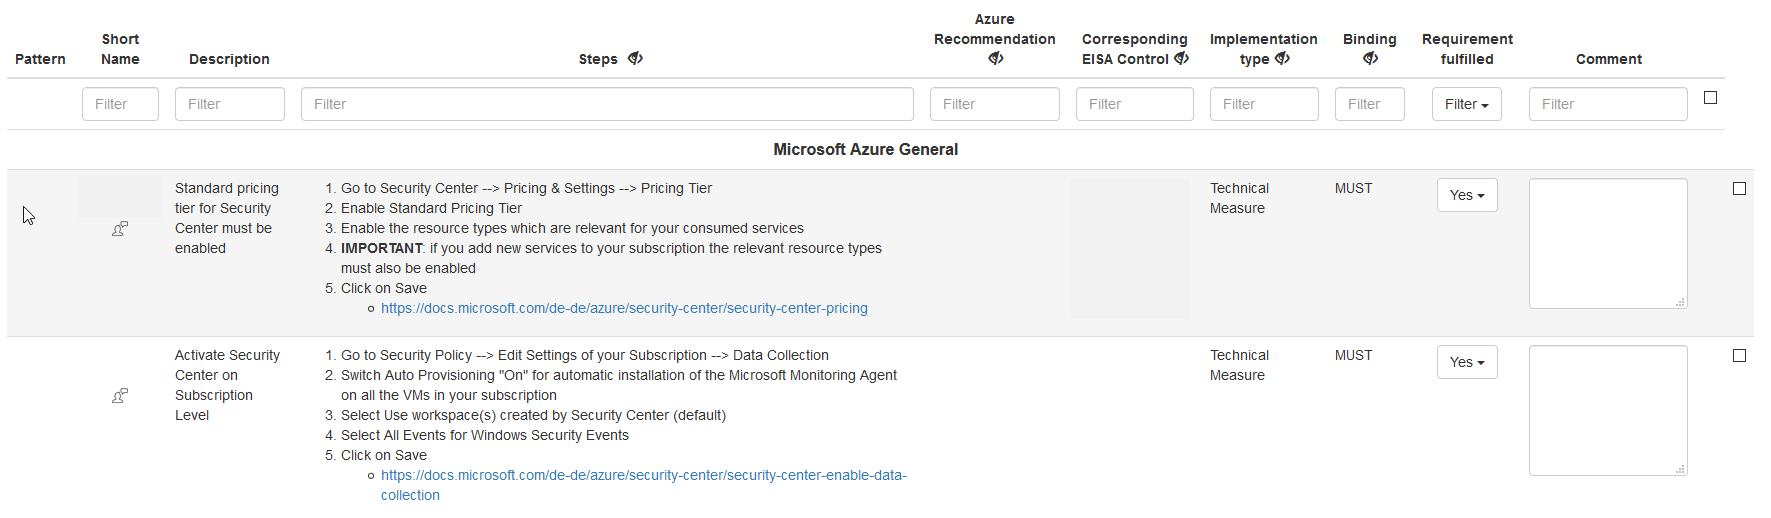
\includegraphics[height=5cm]{secrat_screen.png}
\end{center}
\caption[Screenshot of SecurityRat]{Screenshot of SecurityRAT Microsoft "Azure Implementation Guide" requirements.}
%Source:
\label{fig_devsecops}
\end{figure}

The focus on automation becomes present through the integration of JIRA into the tool. JIRA tickets can automatically be created, tracked, and documented with SecurityRAT.

\begin{figure}[ht!]
\begin{center}
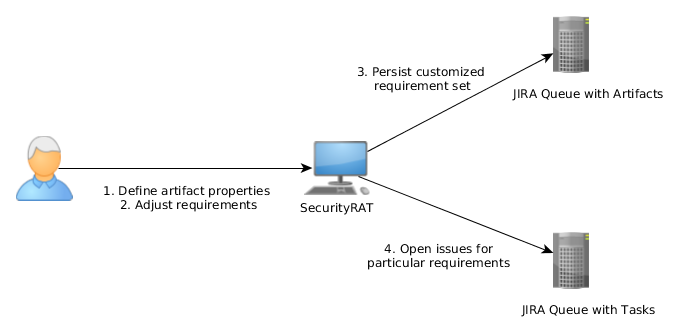
\includegraphics[height=8cm]{security_rat.png}
\end{center}
\caption[SecurityRat Schema]{Schematic drawing of SecurityRAT process flow. Graph from \citep{secrat2020}}
%Source: https://securityrat.github.io/
\label{fig_devsecops}
\end{figure}

\vskip 1cm

The process flow of SecurityRAT can be described as follows:

\begin{itemize}\itemsep0pt \parskip0pt \parsep0pt
    \item Property specification of the software project, called artifact 
    \item Common security requirements are listed as a subset of the given requirements database
    \item Decide which requirements are needed and how they are handled
    \item Create automated JIRA tickets for state tracking of open issues
\end{itemize}

SecurityRAT provides additional automation for project excel sheet export, training slides creation, and with SecurityCAT, automated testing of trivial technical measures.


\section{Adding a Compliance Automation Tool (CAT)}
\label{secCat}
SecurityRAT is a tool designed for the management and handling of security requirements. Even though it has some convenience automation features like the above mentioned excel sheet export, it does not provide automated testing of system compliance to security requirements.

SecurityRAT exposes a REST API that allows to plug in other systems. SecurityCAT is a proof of concept implementation of such a system focused on compliance and security evaluations. It consists of a gateway and several use-case specific microservices that can be used to test the according to requirements automatically. According to the needs, those microservices can be set up or not. The detailed explanation of the structure and architecture of SecurityCAT is described in \ref{architecture}.

\newpage

\begin{figure}[ht!]
\begin{center}
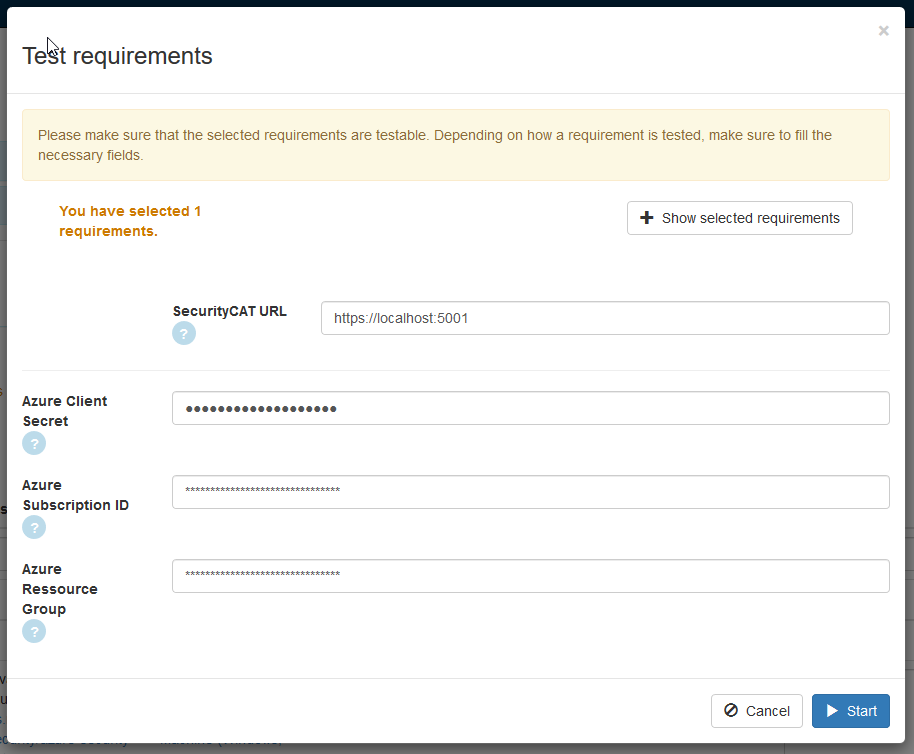
\includegraphics[height=12cm]{secrat_test_requirements_widget.png}
\end{center}
\caption[SecurityRat test execution widget for SecurityCAT]{SecurityRat test execution widget for SecurityCAT}
%Source:
\label{fig_devsecops}
\end{figure}

By jointly incorporating the execution of automated testing into SecurityRAT, the whole process of evaluating a project is meant to be streamlined and parallelized. The figure above shows the test execution widget within SecurityRAT that is used to trigger, and therefore delegate, the execution, and evaluation of the selected requirements. 
To better identify requirements that can be tested in an automated manner, they will get a unique tag that identifies them and therefore make them easy to filter.